\section{迭代选解与隐式偏置}
\label{sec:opt-fit-implicit-bias}

第一节说过，读数看不见的方向要由额外的偏好来确定。前面的偏好都写在目标里。可是在过参数化的拟合中，人们常常不加任何正则，直接用梯度法极小化数据误差；此时目标有无穷多个最小点，或者根本没有有限的最小点，算法还是会交出一个确定的结果。本节研究这个结果由什么决定。由优化过程本身产生、没有写进目标的选择偏好，称为\term{隐式偏差}（implicit bias），也常称隐式偏置。我们先在最小二乘中完整证明它，再以补充的形式说明分类和矩阵因子化中的相应现象及其适用边界。

\subsection{最小二乘中的初值与尺度}
\label{sec:opt-fit-implicit-least-squares}

\paragraph{梯度永远在行空间中}
考虑$F(\bm w)=\frac1{2n}\|\bm X\bm w-\bm y\|_2^2$，$\bm X\in\mathbb R^{n\times d}$可以有$d>n$。它的梯度$\nabla F(\bm w)=\bm X^\top(\bm X\bm w-\bm y)/n$总属于$\operatorname{range}(\bm X^\top)=(\ker\bm X)^\perp$。梯度下降$\bm w^{(t+1)}=\bm w^{(t)}-\eta\nabla F(\bm w^{(t)})$每步只沿行空间移动，所以$\bm w^{(t)}$在$\ker\bm X$上的投影始终等于初值的投影：数据看不见的方向，算法也从不触碰。

\begin{theorem}[梯度下降的最小二乘极限]
\label{thm:opt-fit-gd-limit}
设$\bm X\ne\bm 0$，步长$0<\eta<2n/\|\bm X\|_2^2$。则对任意初值$\bm w^{(0)}$，
\[
  \bm w^{(t)}\to\bm X^\dagger\bm y+P_{\ker\bm X}\bm w^{(0)} .
\]
特别地，零初值时极限是$\bm X^\dagger\bm y$，即所有最小二乘解中欧氏范数最小的一个。
\end{theorem}

\begin{proof}
设$\bm X=\sum_{k=1}^r\sigma_k\bm u_k\bm v_k^\top$，$\sigma_1\ge\cdots\ge\sigma_r>0$，把$\{\bm v_1,\dots,\bm v_r\}$补成$\mathbb R^d$的标准正交基。记坐标$z_k=\bm v_k^\top\bm w$。对$k\le r$，$\bm v_k^\top\bm X^\top(\bm X\bm w-\bm y)=\sigma_k(\sigma_kz_k-\bm u_k^\top\bm y)$，令$z_k^\star=\bm u_k^\top\bm y/\sigma_k$，更新化为
\[
  z_k^{(t+1)}-z_k^\star=\Bigl(1-\frac{\eta\sigma_k^2}n\Bigr)\bigl(z_k^{(t)}-z_k^\star\bigr).
\]
由$0<\eta\sigma_k^2/n\le\eta\sigma_1^2/n<2$，因子的绝对值小于$1$，$z_k^{(t)}\to z_k^\star$。对$k>r$，$\bm v_k\in\ker\bm X$，梯度在该坐标上为零，$z_k^{(t)}=z_k^{(0)}$。合起来，极限为$\sum_{k\le r}z_k^\star\bm v_k+\sum_{k>r}z_k^{(0)}\bm v_k=\bm X^\dagger\bm y+P_{\ker\bm X}\bm w^{(0)}$。$\bm X^\dagger\bm y$是最小范数最小二乘解，见前文引用的卷一“线性方程与矩阵方程”章。
\end{proof}

定理没有假设数据可以被精确插值：$\bm y\notin\operatorname{range}\bm X$时，极限仍是最小二乘解，只是残差不为零。非零初值时，算法选出的是离初值最近的最小二乘解。

\paragraph{预条件改变被选中的解}
把更新改为$\bm w^{(t+1)}=\bm w^{(t)}-\eta\bm P\nabla F(\bm w^{(t)})$，$\bm P$是固定的对称正定矩阵。令$\bm w=\bm P^{1/2}\bm z$，更新变为
\[
  \bm z^{(t+1)}=\bm z^{(t)}-\frac\eta n\bm P^{1/2}\bm X^\top\bigl(\bm X\bm P^{1/2}\bm z^{(t)}-\bm y\bigr),
\]
它是对$\frac1{2n}\|\tilde{\bm X}\bm z-\bm y\|_2^2$（$\tilde{\bm X}=\bm X\bm P^{1/2}$）的普通梯度下降。由定理~\ref{thm:opt-fit-gd-limit}，在$0<\eta<2n/\|\bm X\bm P^{1/2}\|_2^2$时，零初值的$\bm z^{(t)}$收敛到使$\|\bm z\|_2$最小的最小二乘解。$\bm z\mapsto\bm P^{1/2}\bm z$把两组最小二乘解一一对应，且$\|\bm z\|_2^2=\bm w^\top\bm P^{-1}\bm w$，所以$\bm w^{(t)}$收敛到使$\bm w^\top\bm P^{-1}\bm w$最小的最小二乘解。预条件不只改变速度，还改变了被选中的解。

\begin{example}[同一条直线上的两个选择]
\label{ex:opt-fit-implicit-preconditioner}
取$n=1$，$\bm X=(1,1)$，$y=1$，最小二乘解（此处即插值解）是直线$w_1+w_2=1$上的全部点，目标值都为零。$\bm P=\bm I$时，步长条件为$\eta<1$，零初值下的极限是最小欧氏范数解$(\tfrac12,\tfrac12)$。$\bm P=\operatorname{diag}(1,4)$时，步长条件为$\eta<2/5$，极限使$w_1^2+w_2^2/4$最小：由Lagrange条件$2w_1=\nu$、$w_2/2=\nu$得$w_2=4w_1$，再代入约束得$(\tfrac15,\tfrac45)$。
\end{example}

图~\ref{fig:opt-fit-implicit-bias-gd}画出了这两条轨迹。由于梯度总与$(1,1)$成比例，$\bm P=\bm I$的轨迹沿$(1,1)$方向直线前进，在与解直线相切的圆处停下；$\bm P=\operatorname{diag}(1,4)$的轨迹沿$\bm P(1,1)^\top=(1,4)^\top$方向前进，停在与解直线相切的椭圆$w_1^2+w_2^2/4=\tfrac15$上。从$(1.2,-0.5)$出发的绿色轨迹则沿$(1,1)$方向落到$(1.35,-0.35)$，它保留了初值在$\ker\bm X=\operatorname{span}\{(1,-1)^\top\}$上的分量。

\begin{figure}[!htbp]
  \centering
  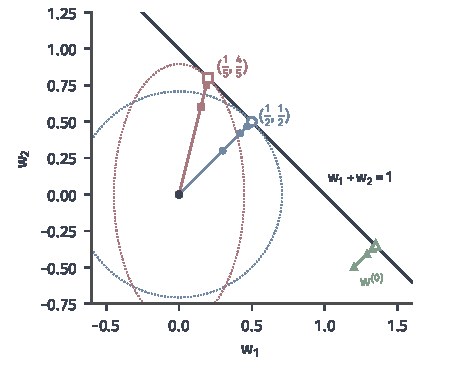
\includegraphics[width=80mm]{figures/03-optimization-evolution-and-signals/01-optimization/matplotlib/c8-implicit-bias-gd/figure.pdf}
  \caption{欠定最小二乘$\tfrac12(w_1+w_2-1)^2$上梯度下降的极限。黑线为全部最小点$w_1+w_2=1$。蓝色轨迹：$\bm P=\bm I$、$\eta=0.3$、零初值，收敛到$(\tfrac12,\tfrac12)$，蓝色点线圆$\|\bm w\|_2^2=\tfrac12$与黑线相切于此；红色轨迹：$\bm P=\operatorname{diag}(1,4)$、$\eta=0.15$、零初值，收敛到$(\tfrac15,\tfrac45)$，红色点线椭圆$w_1^2+w_2^2/4=\tfrac15$与黑线相切于此；绿色轨迹：$\bm P=\bm I$、初值$(1.2,-0.5)$，收敛到$(1.35,-0.35)$。标记为前几次迭代，空心标记为极限。}
  \label{fig:opt-fit-implicit-bias-gd}
\end{figure}

\paragraph{隐式选择不等于显式正则化}
零初值梯度下降的极限$\bm X^\dagger\bm y$恰好是岭回归解在$\lambda\downarrow0$时的极限，但这并不意味着两者在其他参数下也一致。仍以$\bm X=(1,1)$、$y=1$为例，$\lambda=1$的岭回归解是$(\bm X^\top\bm X+\bm I)^{-1}\bm X^\top y=(\tfrac13,\tfrac13)$，它根本不是最小二乘解；梯度下降在任何有限步停下的点也与任何一个$\lambda$的岭回归解一般不重合，除非像本例这样整条轨迹恰好落在同一条射线上。隐式偏好描述的是“算法在最小点集合中选哪一个”，显式正则化则改变了最小点集合本身。

\subsection{可分分类中的方向选择（补充）}
\label{sec:opt-fit-separable}

\paragraph{没有有限的最小点}
在二分类中，数据$(\bm x_i,y_i)$，$y_i\in\{-1,1\}$，用齐次线性预测器$\bm w^\top\bm x$与logistic损失，目标为
\[
  F(\bm w)=\frac1n\sum_{i=1}^n\log\bigl(1+\exp(-y_i\bm w^\top\bm x_i)\bigr).
\]
设数据严格线性可分，即存在$\bar{\bm w}$使$y_i\bar{\bm w}^\top\bm x_i>0$对所有$i$成立。沿这个方向放大参数，$F(s\bar{\bm w})\to0$（$s\to\infty$）；而每一项都严格为正，任何有限的$\bm w$都有$F(\bm w)>0$。所以下确界$0$达不到，问题没有有限的最小点，梯度下降的参数范数必然趋于无穷。这时有意义的问题不再是“参数收敛到哪个最小点”，而是“参数的方向趋于哪里”。

\paragraph{方向趋于硬间隔解}
Soudry等人证明\scite{soudry2018implicit}：在上述设定下，对欧氏全批量梯度下降，取充分小的固定步长（例如小于$2/\beta$，$\beta$为$F$梯度的Lipschitz常数，对logistic损失可取$\|\bm X\|_2^2/(4n)$，$\bm X$的行是$\bm x_i^\top$），从任意初值出发，都有$\|\bm w^{(t)}\|_2\to\infty$且
\[
  \frac{\bm w^{(t)}}{\|\bm w^{(t)}\|_2}\to\frac{\hat{\bm w}}{\|\hat{\bm w}\|_2},\qquad
  \hat{\bm w}=\argmin_{\bm w}\Bigl\{\|\bm w\|_2^2:\ y_i\bm w^\top\bm x_i\ge1,\ i=1,\dots,n\Bigr\}.
\]
$\hat{\bm w}$是\term{硬间隔}（hard margin）支持向量机的解：在所有把每个样本的间隔推到至少$1$的方向中，它的范数最小，也就是几何间隔最大。方向收敛只以对数速率进行，非常缓慢。

图~\ref{fig:opt-fit-separable}给出一个六点的例子。硬间隔解为$\hat{\bm w}=(0.8,0.4)$，唯一的支持向量是$(-1,-0.5)$。从零初值、步长$\eta=1$出发（这里$\|\bm X\|_2^2/(4n)\approx1.66$，步长满足$\eta<2/\beta$），迭代方向与$\hat{\bm w}$的夹角在第$1$步约为$25^\circ$，第$1701$步约为$11.6^\circ$，到第$10^6$步仍有约$5.9^\circ$，此时$\|\bm w^{(t)}\|_2\approx11.0$。迭代次数每增加数十倍，夹角才减少几度。

\begin{figure}[!htbp]
  \centering
  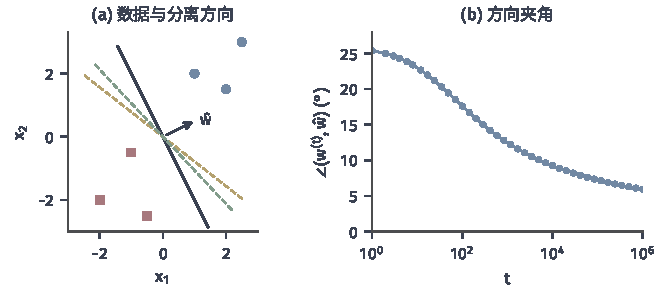
\includegraphics[width=112mm]{figures/03-optimization-evolution-and-signals/01-optimization/matplotlib/c8-separable-direction/figure.pdf}
  \caption{可分数据上logistic损失梯度下降的方向。(a)~正类（蓝色圆点）与负类（红色方块）各三个点；黑线为硬间隔解$\hat{\bm w}=(0.8,0.4)$对应的分界线，箭头为$\hat{\bm w}$的方向；黄色与绿色虚线为第$1$步与第$143$步迭代对应的分界线。(b)~迭代方向与$\hat{\bm w}$的夹角随迭代次数（对数刻度）的变化，零初值，$\eta=1$。}
  \label{fig:opt-fit-separable}
\end{figure}

\paragraph{结论的边界}
这个结论绑定于齐次线性预测器、指数型尾部的损失（logistic、指数损失）和欧氏梯度下降。换成尾部更重的损失、加入预条件或改用自适应方法，极限方向一般不同，需要重新分析。它只描述优化在无穷多个“近似最小点”中选择了什么，不直接给出测试误差；间隔与泛化的关系属于学习理论的内容。

\subsection{参数化、秩约束与谱选择的边界（补充）}
\label{sec:opt-fit-factorization}

\paragraph{因子化先规定了可表达的范围}
设要拟合的未知量是矩阵$\bm W\in\mathbb R^{p\times q}$。直接优化$\bm W$与写成$\bm W=\bm U\bm V^\top$（$\bm U\in\mathbb R^{p\times k}$，$\bm V\in\mathbb R^{q\times k}$）再优化因子，是两个不同的问题。内部宽度$k$先规定了$\operatorname{rank}\bm W\le k$：这是显式的低秩候选集合，属于表达限制，不是算法的偏好。参数化还引入了冗余：$(c\bm U,\bm V/c)$对任何$c\ne0$都给出同一个$\bm W$，就像核系数沿$\ker\bm G$移动不改变函数一样。

\paragraph{因子上的惩罚是一种显式偏好}
在因子上加平方惩罚，等价于在$\bm W$上加核范数（奇异值之和）$\|\bm W\|_*$惩罚：当$k\ge\operatorname{rank}\bm W$时，
\[
  \|\bm W\|_*=\min_{\bm U\bm V^\top=\bm W}\ \frac12\bigl(\|\bm U\|_F^2+\|\bm V\|_F^2\bigr).
\]
证明如下。设$\bm W=\bm A\bm\Sigma\bm B^\top$是紧奇异值分解，$\bm A,\bm B$的列标准正交。对任何$\bm U\bm V^\top=\bm W$，$\|\bm W\|_*=\operatorname{tr}(\bm A^\top\bm W\bm B)=\langle\bm U^\top\bm A,\bm V^\top\bm B\rangle_F\le\|\bm U^\top\bm A\|_F\|\bm V^\top\bm B\|_F\le\|\bm U\|_F\|\bm V\|_F\le\tfrac12(\|\bm U\|_F^2+\|\bm V\|_F^2)$，其中第二个不等号用了$\bm A$、$\bm B$的列标准正交。取$\bm U=\bm A\bm\Sigma^{1/2}$、$\bm V=\bm B\bm\Sigma^{1/2}$（宽度不足$k$时补零列）各处取等。所以“因子化加权重衰减”是一个显式的核范数正则化问题，它与“不加惩罚、靠迭代形成的偏好”应当分开讨论。

\paragraph{因子化本身不保证低秩}
没有显式惩罚时，因子化的梯度法是否偏向低秩或小核范数，取决于初值、步长与问题结构，不能仅凭“用了因子化”下结论。一个例子：$F(\bm U,\bm V)=\tfrac12\|\bm U\bm V^\top-\bm I_2\|_F^2$，取$\bm U^{(0)}=\bm V^{(0)}=a^{(0)}\bm I_2$，$0<a^{(0)}<1$。对$\bm U$的梯度是$(\bm U\bm V^\top-\bm I)\bm V=(a^2-1)a\bm I$，对$\bm V$相同，所以梯度下降保持$\bm U=\bm V=a^{(t)}\bm I$，$a^{(t+1)}=a^{(t)}-\eta(a^{(t)2}-1)a^{(t)}$。当$0<\eta<\tfrac12$时，映射$a\mapsto a+\eta a(1-a^2)$在$[0,1]$上严格递增且以$1$为不动点，$a^{(t)}$单调增加并收敛到$1$，乘积始终是满秩矩阵$a^2\bm I_2$，最终等于秩为$2$的$\bm I_2$。正面的结论都附带条件：例如Gunasekar等人在测量矩阵两两可交换等条件下，对半正定因子化的梯度流，证明了“先让时间趋于无穷、再让初始化尺度趋于零”的顺序极限给出最小核范数解\scite{gunasekar2017matrix}；交换条件与顺序极限都是定理的组成部分。

\paragraph{留给后续的问题}
由此提出的一般问题是：哪些初始条件与更新规律，会使迭代偏向哪些谱方向？回答它通常要研究连续时间的梯度流及其在奇异值上的演化，例如深线性网络在平衡初始化下的奇异值动力学，以及非线性网络中低秩倾向的反例。这些属于轨迹分析，在本卷“过程与轨迹演化”部分（从第~\ref{chap:dynamical-systems-and-state-estimation}章开始）的动力系统语言下展开，具体网络结构则在模型部分讨论。本节只确定判断的对象与条件：同样的数据目标，不同的参数化、初值和算法，可以选出不同的解。
